%% Preambel
\documentclass[conference,compsoc,final,a4paper]{IEEEtran}
\usepackage[utf8]{inputenx}

\newcommand{\autoren}[0]{Salame, Ahmed}
\newcommand{\dokumententitel}[0]{Wieso ein gutes API Design wichtig ist}

% Hie muss normalerweise nichts angepasst werden
\usepackage[pdftex]{graphicx}
\graphicspath{{img/}}
\DeclareGraphicsExtensions{.pdf,.jpeg,.png}
\usepackage[cmex10]{amsmath}
\usepackage{algorithmic}
\usepackage{array}
\usepackage{dblfloatfix}
\usepackage{url}
\usepackage[autostyle=true,german=quotes]{csquotes}
\usepackage[backend=biber]{biblatex}
\usepackage{booktabs}
\usepackage{xcolor}
\usepackage{listings}             % Source Code listings
\usepackage[printonlyused]{acronym}

% Farben definieren
\definecolor{linkblue}{RGB}{0, 0, 100}
\definecolor{linkblack}{RGB}{0, 0, 0}
\definecolor{darkgreen}{RGB}{14, 144, 102}
\definecolor{darkblue}{RGB}{0,0,168}
\definecolor{darkred}{RGB}{128,0,0}
\definecolor{comment}{RGB}{63, 127, 95}
\definecolor{javadoccomment}{RGB}{63, 95, 191}
\definecolor{keyword}{RGB}{108, 0, 67}
\definecolor{type}{RGB}{0, 0, 0}
\definecolor{method}{RGB}{0, 0, 0}
\definecolor{variable}{RGB}{0, 0, 0}
\definecolor{literal}{RGB}{31,0, 255}
\definecolor{operator}{RGB}{0, 0, 0}

\usepackage[ngerman]{betababel}
\usepackage[
	    unicode=true,
      hypertexnames=false,
      colorlinks=true,
      colorlinks=false,
      linkcolor=darkblue,
      citecolor=darkblue,
      urlcolor=darkblue,
      pdftex
   ]{hyperref}
%	 \PrerenderUnicode{ü}

% Einstellungen für Quelltexte
\lstset{
      xleftmargin=0.1cm,
      basicstyle=\scriptsize\ttfamily,
      keywordstyle=\color{keyword},
      identifierstyle=\color{variable},
      commentstyle=\color{comment},
      stringstyle=\color{literal},
      tabsize=2,
      lineskip={2pt},
      columns=flexible,
      inputencoding=utf8,
      captionpos=b,
      breakautoindent=true,
	  breakindent=2em,
	  breaklines=true,
	  prebreak=,
	  postbreak=,
      numbers=none,
      numberstyle=\tiny,
      showspaces=false,      % Keine Leerzeichensymbole
      showtabs=false,        % Keine Tabsymbole
      showstringspaces=false,% Leerzeichen in Strings
      morecomment=[s][\color{javadoccomment}]{/**}{*/},
      literate={Ö}{{\"O}}1 {Ä}{{\"A}}1 {Ü}{{\"U}}1 {ß}{{\ss}}2 {ü}{{\"u}}1 {ä}{{\"a}}1 {ö}{{\"o}}1
}

\hypersetup{
  pdftitle={\dokumententitel},
	pdfauthor={\autoren},
	pdfdisplaydoctitle=true
}

% Wo liegt Sourcecode?
\newcommand{\srcloc}{src/}

% Literatur einbinden
\addbibresource{literatur.bib}

\begin{document}

% Titel des Dokuments
\title{\dokumententitel}

% Namen der Autoren
\author{
  \IEEEauthorblockN{\autoren}
  \IEEEauthorblockA{
    Hochschule Mannheim\\
    Fakultät für Informatik\\
    Paul-Wittsack-Str. 10,
    68163 Mannheim
    }
}

% Titel erzeugen
\maketitle
\thispagestyle{plain}
\pagestyle{plain}
 % Weitere Einstellungen aus einer anderen Datei lesen

% Eigentliches Dokument beginnt hier
% ----------------------------------------------------------------------------------------------------------

% Kurze Zusammenfassung des Dokuments
\begin{abstract}
--TODO--\\
Dieses Paper soll aufzeigen was eine \ac{API} ist und was daran wichtig ist für einen Entwickler. Dabei zeigt dieses Paper Kriterien für ein gutes \ac{API} Design. Es zeigt ebenso was schlechtes Design ausmacht anhand von Beispielen. Es werden verschiedene Ansätze aufgezeigt, wie ein nutzerfreundlicheres \ac{API} entworfen werden kann.

\end{abstract}

\tableofcontents

% ANMERKUNGEN
% Einheitliche Bezeichungen "Entwickler" stattt "Nutzer"
\section{Einleitung}

Application Programming Interfaces(API) sind kaum wegzudenken. So gut wie alle Programmbibliotheken, Frameworks und \ac{SDK} nutzen eine API. Auf der Webseite programmableweb\footnote{https://www.programmableweb.com/} werden allein über 18.000 unterschiedliche APIs aufgelistet.

Für die Entwicklung neuer APIs gibt es ein immer größer werdender Markt für Firmen, die aktiv bei der Entwicklung der APIs bei anderen Unternehmen aushelfen, wie Apigee \footnote{https://apigee.com/api-management/}.

Zudem besitzen Firmen unterschiedliche Strategien, wie sie mit ihren APIs umgehen \cite[siehe Seite 11]{spichale2017}. 
So hat der Blogging-Dienst Twitter seine Popularität unter anderem durch dessen gute API zu verdanken. Es bot die notwendige Infrastruktur, so dass Twitter auf unzähligen Endgeräte genutzt werden konnte. Facebook setzt mit ihrer API auf ausfallsicher und Skalierbarkeit. Oder die Firma Best Buy entwickelte eine API, um ihren Online-Dienst weiter auszubauen. 


\section{Application Programming Interface}


\subsection{Die Definition einer \ac{API}}

Eine \ac{API} besitzt keine einheitliche Definition. Die unterschiedlichen Erklärungsansätze weichen an bestimmten Punkten voneinander ab. So beschreibt Reddy \cite{reddy2011}, dass eine API Schnittstellen hat, die eine Abstraktion eines Problems darstellen und wie Entwickler diese Nutzen, um das bestehendes Problem zu lösen.
Blochs Definition ist dabei etwas Allgemeiner. Laut Bloch \cite{bloch2014} handelt es sich um eine \ac{API}, wenn es folgende Kriterien erfüllt:
\begin{enumerate}
\item Eine API bietet eine Menge an Operationen an, welche durch ihre Eingaben und Ausgaben definiert sind.\\
\item Es ist möglich die Schnittstellen neu zu implementieren, ohne dass der Nutzer seinen Code anpassen muss.
\end{enumerate}

Allgemein kann eine \ac{API} als etwas beschrieben werden, dass dem Nutzer zur Verfügung gestellt wird, so dass dieser darüber mit einem Softwaresystem kommunizieren kann.
Im folgenden Paper wird diese Definition zugrunde gelegt.\\
Folgende beispielhafte Java Methode soll verdeutlichen, wie eine Schnittstelle konkret aussehen kann:

\begin{lstlisting}[language=Java,caption=Beispiel einer Schnittstelle]

public String linkStrings(String head , String tail);

\end{lstlisting}

Der Name der Schnittstelle lautet linkStrings, ihre Eingaben sind Zwei Strings, mit den Bezeichnern head und tail. Bei der Ausgabe der Methode handelt es sich um den Rückgabewert, welches in diesem Fall als Typ auch ein String ist. Die eigentliche Implementierung ist dabei für den Entwickler, der diese Schnittstelle nutzt, nicht wichtig. Der Entwickler benötigt zum nutzen der Schnittstelle, ausschließlich die Schnittstelle selbst.


\subsection{Die Arten einer API}

Es gibt unterschiedliche Arten einer API \cite{myers2016}. Es ist möglich eine API grob in drei Kategorien einzuteilen. Interne APIs sind nicht für die Öffentlichkeit gedacht. Sie werden intern verwendet und sind daher nicht auf die Akzeptanz der Community angewiesen. Dies sorgt dafür, dass sie nicht den strengen Regeln befolgen müssen, die eine API ausmacht. Es ist möglich noch Änderungen vorzunehmen an der Schnittstelle. Sie helfen dabei, interne Strukturen umzusetzen, wie das arbeiten in verschiedenen Teams. 

Öffentliche APIs sind der Öffentlichkeit zugänglich. Sobald eine API öffentlich zugreifbar ist, ist es kaum möglich diese nachhaltig so abzuändern, ohne dass all die Nutzer dieser API auch ihren Code anpassen müssen. Zu einer guten Öffentlichen API gehört auch eine dazu passende Dokumentation. Beispiele hierfür wäre das \ac{JDK} von Java oder die \ac{STL} von C.

Neben der Öffentlichen und Internen API gibt es noch die Remote APIs. Hier werden die Schnittstellen über das Netzwerk zugänglich gemacht. Für den Entwickler soll dabei das Gefühl entstehen, dass die Nutzung der API lokal geschieht. Beispiel hierfür wäre die Remote API von Java.


\subsection{Die Vorteile einer API}

Es gibt viele gute Gründe \ac{API}s zu nutzen. Nach Reddy \cite{reddy2011} sprechen insbesondere folgende Gründe für das nutzen einer API:

\begin{description}
\item [Robustheit] \hfill \\

Eine \ac{API} sorgt für robusteren Code. Da die Nutzer nur über eine Schnittstelle mit den System Kommunizieren, besteht Information Hiding. Es sorgt dafür, dass die eigentliche Implementation ausgetauscht werden kann, ohne das es beim Nutzer angepasst werden muss. So lässt sich ganz leicht die bestehende Implementierung austauschen, ohne das der Nutzern dieser API gezwungen ist, seinen Code Anpassung zu müssen.\\

\item [Parallele Entwicklung]\hfill \\

Wenn ein Entwickler ein Programm schreiben möchte und dazu den Code von einem anderen Entwickler braucht, dessen Code allerdings nicht fertig ist, wäre es verschwendete Zeit, falls einer auf die Fertigstellung des Codes warten muss. Es wäre klüger wenn stattdessen sich beide einigen würden, wie die Schnittstellen auszusehen haben. So könnte man von der Implementierung der Schnittstelle ein Mockup erstellen und in ihrem Inhalt einfache Werte zurückgeben, so dass sich der Code zumindest Compilieren lässt. Die eigentliche Implementierung kann so später stattfinden, so dass der Nutzer dieser Schnittstelle nur wenige Änderung, bis keine Änderung vornehmen muss.
\\
So lässt es sich realisieren, dass mehrere Teams parallel Entwickeln können, ohne jedes Detail von den Aufgaben der anderen Teams zu kennen.\\
	
\item [Wiederverwendbarkeit]\hfill \\
	
Eines der größten Vorteile einer API ist die Wiederverwendbarkeit von bisher existierenden Code. Das Entwickeln von eigenen Schnittstellen kostet sehr viel Zeit und Geld.
Durch das wiederverwenden von \ac{API}, ob nun eigene oder von anderen, kann man sich dies einsparen. Dabei stehen sowohl kostenpflichtige, als auch kostenlose zur Auswahl. Es existieren viele unterschiedliche \ac{API}s für die unterschiedlichsten Probleme.

Es gibt als Beispiel viele APIs, die sich mit dem laden von Bildern beschäftigen\footnote{http://cimg.eu/}. Viele solcher Bibliotheken haben bereits einen gewissen Reifeprozess durchgemacht. Sie wurden ausgiebig getestet und haben womöglich auch ein breites Spektrum an Informationen. Als Beispiel ist hier die Spiele-Bibliothek LibGDX zu nennen. Es hat eine große Community, an die sich Entwickler wenden können, falls sie fragen haben\footnote{http://www.badlogicgames.com/forum/}.
\end{description}

Zusätzlich schreibt Spichale, dass mithilfe von gutem API Design es einfacher ist, dass die Entwickler, welche diese Schnittstellen letztendlich Implementieren, es einfacher haben ihren Code sauber zu halten, so dass sie dem Allgemeinen stand vom Clean Code entspreche \cite[siehe Seite 39]{spichale2017}.


\section{Beispiele von Schlechten API Design}

Es gibt sehr viele Programmbibliotheken, die sehr viele Schnittstellen anbieten, auf welche die Entwickler zugriff haben. Bei einer Erweiterung der Bibliothek kommen zudem immer mehr Schnittstellen hinzu. Wo in dem \ac{JDK} aus Java 8 sich noch 4240 Klassen befinden\footnote{https://docs.oracle.com/javase/8/docs/api/}, hat dessen Nachfolger Java 9 bereits 6005 Klassen \footnote{https://docs.oracle.com/javase/9/docs/api/}. Bei einer solch wachsenden Anzahl an Klassen ist es wichtig sich ein Konzept auszudenken, damit der Entwickler bei der Bibliothek keine Schwierigkeiten bekommt. Wenn einzelne Punkte nicht eingehalten werden, kann der Entwickler schnell die Überblick verlieren. Der Erfolg einer Bibliothek kann unter anderem dadurch gemessen werden, wie häufig sie von Verschiedenen Entwicklern genutzt wird. In diesem Kapitel werden Punkte aufgezählt, die den Erfolg einer Bibliothek bestimmen können.


\subsection{Mangelnde Dokumentation}\label{MD}

Die Dokumentation einer Bibliothek beschreibt ihre Funktionalität, auf die der Entwickler zugreifen kann. So werden die Schnittstellen der Bibliothek hier definiert, sowie mit einer zusätzlichen Beschreibung versehen. Zusätzlich kann eine Dokumentation noch weitere Punkte beinhalten, wie Namens Konventionen. Ein bekanntes Beispiel hierfür ist die Java Dokumentation von Oracle. Hier werden alle Klassen auf die ein Entwickler Zugriff hat angezeigt. Neben einer Beschreibung der Klassen, gibt es in der Java API Dokumentation auch  eine Beschreibung für die Methoden einer Klasse.

Für das erstellen von Dokumentation gibt es viele Möglichkeiten. Die Programmiersprache Java bietet für die Dokumentation des Quellcodes das Javadoc an \cite{oracle2017}. Bei Javadoc handelt es sich um ein Tool für das Generieren von API Dokumentation. Dabei braucht ein Entwickler z.B. über einer Methode nur ein Javadoc Kommentar zu schreiben, so dass das Javadoc Tool es in \ac{HTML} code umwandeln kann. Beim Javadoc Kommentar lassen sich auch die Abhängigkeiten als Referenzen zu anderen Klassen und Methoden herstellen, das erleichtert dem Entwickler zusätzlich die Suche nach der benötigten Klassen. Die Java API Dokumentation z.B. wurde so erstellen. Folgend wird eine Methode mitsamt deren Javadoc aus der java.lang.String Klasse gezeigt:

\begin{lstlisting}[language=Java,caption=Beispiel eines Javadoc Kommentars]

  /**
  * Returns the {@code char} value at the
  * specified index. An index ranges from {@code 0} to
  * {@code length() - 1}. The first {@code char} 
  * value of the sequence
  * is at index {@code 0}, the next at index {@code 1},
  * and so on, as for array indexing.
  *
  * <p>If the {@code char} value specified by the 
  * index is a
  * <a href="Character.html#unicode">surrogate</a>, 
  * the surrogate
  * value is returned.
  *
  * @param      index   the index of the {@code char} 
  * 					value.
  *
  * @return     the {@code char} value at the specified 
  *				index of this string.
  *             The first {@code char} value is at 
  *				index {@code 0}.
  *
  * @exception  IndexOutOfBoundsException  if 
  *				the {@code index}
  *             argument is negative or not less than 
  *				the length of this string.
  */
 public char charAt(int index) {
     if ((index < 0) || (index >= value.length)) {
         throw 
         	new StringIndexOutOfBoundsException(index);
     }
     return value[index];
 }

\end{lstlisting}

Auch andere Bibliotheken, die in Java geschrieben worden sind, haben so ihre Dokumentation erstellt, wie die Bibliothek \ac{LWJGL} \footnote{https://javadoc.lwjgl.org/}. Das Javadoc nimmt beim erstellen des Quellcodes viel Arbeit für eine externe Dokumentation ab. 

Ein Ähnliches Tool für das erstellen für die Dokumentation ist Doxygen \cite{dimitri2017}. Doxygen steht dabei nicht nur für Java zur Verfügung, sondern auch für andere Programmiersprachen wie C, C++ oder Python. Wie in Javadoc wird auch hier die Dokumentation über Kommentare im Quelltext gesteuert, allerdings hat der Entwickler in Doxygen die Möglichkeit die Dokumentation in verschiedenen arten anzugeben \footnote{https://www.stack.nl/~dimitri/doxygen/manual/docblocks.html}. Es ist zudem möglich mit Doxygen einen zusammenfassenden Überblick über den Aufbau des Projektes zu erzeugen. Doxygen als Erweiterung wird von vielen Entwicklungsumgebungen\ref{IDE} unterstützt. Es existiert Syntaxhervorhebung. 

Der Vorteil einer Dokumentation welches im Quelltext beschrieben wird, ist dass eine externe Dokumentation fehleranfälliger ist. Zudem ist die Pflege im Quelltext selber einfacher. 


\subsection{Keine Eindeutigen Bezeichnungen von Schnittstellen}

Falls eine Dokumentation die API nicht gut genug Dokumentiert, so dass z.B. eine Methode nicht genau beschrieben wird wie sie intern Funktioniert, kann es dazu führen, dass ein Entwickler eine Schnittstelle der API falsch nutzt.  

%Negatives Beispiele
Die Java Klasse java.util.Calendar \footnote{https://docs.oracle.com/javase/7/docs/api/java/util/Calendar.html} besitzt folgende Methode:

\begin{lstlisting}[language=Java,caption=Signatur der Methode set]

public final void set(int year, int month, int date)

\end{lstlisting}

Anhand der Parameter wäre es naheliegend, das beim Aufruf mit dem folgenden Werten die Methode das Datum auf den 22 August 2017 setzt:

\begin{lstlisting}[language=Java,caption=Setzten eines Datums]

Calendar cal = Calendar.getInstance();

cal.set(2017, 8, 22);

\end{lstlisting}

Allerdings sieht man anhand der Beschreibung der Methode das bei der Eingabe vom Monat, der Januar nicht mit der Eins sondern mit der Null beginnt. Also wäre das Datum, das im obigen Beispiel gesetzt wurde, der 22 September 2017. Vorgesehen ist es, es folgendermaßen zu machen:

\begin{lstlisting}[language=Java,caption=Setzten eines Datums mit Konstante]

Calendar cal = Calendar.getInstance();

cal.set(2017, Calendar.AUGUST, 22);

\end{lstlisting}

Es wird keine Zahl der Methode als Monat übergeben, sondern eine Konstante. Auch wenn die Methode set(...) dokumentiert ist, so liegt die Benennung ihrer Parameter nahe dass der Entwickler, beim nutzen dieser Methode, ihr einfach Zahlen übergeben kann, und er so die Dokumentation nicht zu lesen braucht. Tatsächlich soll laut Bloch \cite{bloch2006} eine Methoden so funktionieren, dass es einfach ist sie zu nutzen, aber schwierig, die Methode falsch zu nutzten. Idealerweise verhindert man das Falsche nutzen einer Methode komplett. Zudem soll eine Methode einer API nicht zwangsweise Dokumentiert sein, wenn der Bezeichner der Methode und ihre Parameter das Nutzen nahelegen. 

Ein anderes Beispiel für eine Methode, die zum Missverständnis führen kann \cite[ab Minute 7]{bloch2009}, ist folgende Methode:

\begin{lstlisting}[language=Java,caption=getBoolean methode aus java.lang.Boolean]

public static boolean Boolean.getBoolean(String name);

\end{lstlisting}

Sie stammt aus der Klasse java.lang.Boolean \footnote{https://docs.oracle.com/javase/9/docs/api/java/lang/Boolean.html}. In Java gibt es Wrapperklassen, die Objekte der primitiven Datentypen darstellen, wie int, double oder auch boolean. Daher gibt es jeweils für jeden Primitiven Datentyp eine Wrapperklasse, für den Datentyp int wäre es z.B. java.lang.Integer. Jede Klasse besitzt eine Methode, dessen Name mit set anfängt, so wie setInteger oder wie im Beispiel setBoolean. Es liegt nahe, dass viele Entwickler zunächst annehmen würden, das beim Aufruf der Methode getValue der Wert true geliefert wird.

\begin{lstlisting}[language=Java,caption=Beispiel mit getValue]

public static boolean getValue(){
	
	boolean bol = Boolean.getBoolean("true");

	if(bol == true){

		return true;

	}else{

		return false;
	
	}
	
}

\end{lstlisting}

Allerdings wird hier false geliefert. In der Dokumentation dieser Methode ist zu entnehmen, dass die Methode getBoolean nur dann true liefert, falls es ein System Property gibt, welches den Name hat und den wert true oder TRUE zugewiesen bekommen hat, den diese Methode als String bekommt:

\begin{lstlisting}[language=Java,caption=Beispiel mit getValue mit vorher gesetztem Propertie]

public static void main(String[] args) {

	Properties properties = new Properties();

	properties.setProperty("TRUE", "true");

	System.setProperties(properties);

	System.out.println(getValue("TRUE")); 

}

public static boolean getValue(String str) {

	boolean bol = Boolean.getBoolean(str);

	if (bol == true) {

		return true;

	} else {

		return false;

	}

}

\end{lstlisting}


Diese Vorgehensweise ist irreführend, da vom Bezeichner der Methode nicht hervorgeht, dass vorher die System Propertie gesetzt werden muss.


\subsection{Factory Pattern bedacht einsetzen}

Das Factory Pattern ist ein Entwurfsmuster, welches von der Gang of Four im Buch Design Pattern beschrieben wird \cite{gamme1995}. Es wird dazu genutzt, dass der Entwickler, um eine Klasse zu instanziieren, es nicht über den Konstruktor tätigt, sondern über eine Methode. Der Entwickler soll so nicht mit dem Konstruktor in Berührung kommen. Es hat insbesondere den Vorteil, dass es so möglich ist, den Typ eines Objektes zur Laufzeit zu bestimmen.
Folgender Codeausschnitt soll eine beispielhafte Implementierung in Java zeigen:

\begin{lstlisting}[language=Java,caption=Beispiel eines Factory Patterns in Java]

public class Factory
{
    public static Base factoryMethod(int typeNumber)
    {
        switch (typeNumber)
        {
            case 1: return new ConcreteProduct1();
            case 2: return new ConcreteProduct2();
            default: throw new ArgumentException("Invalid type.", "type");
        }
    }
}
 
public abstract class Base { }
 
public class ConcreteBase1 extends Base { }
 
public class ConcreteBase2 extends Base { } 

\end{lstlisting}

In dem obigen Code Beispiel werden über die Klasse Factory, die Objekte für die Klasse ConcreteBase1 und ConcreteBase2 erzeugt. So kann der Entwickler, der diese Klassen benötigt, sie nicht nur über die eigentliche Klassen erzeugen, sondern auch vorgefertigte über die statische Methode factoryMethod in der Klasse Factory. So braucht der Entwickler sich keine Gedanken zu machen, welche Parameter der Konstruktor benötigt, falls dieser welche hat.

Auch wenn das Factory Pattern scheinbar dem Entwickler es einfacher macht, an Objekte von einem Bestimmten Typ zu kommen, sollte das Factory Pattern nur bedacht eingesetzt werden. 
In einer Empirischen Studie von Ellis \cite{ellis2007} wurde der Unterschied zwischen einer API die Konstruktoren nutzt und einer API die das Factory Pattern nutzt untersucht. Diese Studie kam zum schluss, dass das Factory Pattern wohl weniger geeignet ist, im gegensatz zu anderen Patterns, wie das Class Cluster Pattern. 


\section{Ansätze zur Verbesserung allgemeiner \ac{API}s}

Eine API bietet viele Möglichkeiten für eine stetige Verbesserung. Eine API, die öffentlich genutzt wird, hat meist viele Schritte zur Verbesserung durchgemacht. Die Schritte zur vermeintlichen Verbesserung einer API kann sich dabei auch über Jahre strecken. Jedoch muss das Resultat nicht zwingend in jedem Fall Positiv sein \cite[siehe Seite 25]{spichale2017}.
\\
Folgend werden einige Vorgehensweisen beschrieben, die Aufzeigen sollen, wie dafür gesorgt werden kann, das eine API auch eine Konsequente Verbesserung widerfährt.


\subsection{Umdenken der Menschen}

--TODO-- Hier soll es einen Ansatz geben, der sich damit befasst, dass man die usability einer API nicht unterschätzen sollte. Viele nehmen das nicht ernst und entwickeln nicht sorgfältig genug. 

\subsection{Nutzer freundlicheres Design}

--TODO-- Hier soll es eine erklärung geben, was genau die meisten Nutzer etwas als besonders benutzerfreundlich betrachten. Dabei soll auch Beispiele aufgezeigt werden, wie man sowas ermittelt


\subsection{APIs Testen}

--TODO--

\section{Ausgewählte \ac{API} Entwurfs Beispiele}

Bloch beschreibt die Eigenschaft einer Gute API folgendermaßen:
\\\\
Good APIs create long-term customers; bad ones create long-term support nightmares\cite{bloch2006}.
\\\\
Eine API, die Nutzerfreundlich ist, erspart einem Entwickler, der diese API nutzt, sehr viel Stress und vor allem Zeit. Auch ist das Design entscheidend für den Erfolg einer API. Viele Entwurfs Beispiele haben sich dabei durchgesetzt, mit dessen Hilfe eine API da hingehend verbessert werden kann, indem es dem Entwickler, welcher mit der API arbeiten muss, das leben erleichtert.

Folgend werden einige Entwurfs Beispiele für eine API aufgezählt.


\subsection{Sinnvolle Klassennamen wählen}

In Programmiersprachen die Objektorientiert sind, wie Java oder C++, sind die Namen der Klassen ebenso Relevant wie die Methodennamen. In reine Objektorientierte Sprache ist es umso wichtiger, da die Objekte alle Schnittstellen nach außen anbieten, auf die dann der Nutzer dieser API zugriff hat. Zudem sind viele Objekte, ob durch Vererbung oder weil bei einer Methode als Parameter erwartet, miteinander Verbunden. 
Der Name einer Klasse sollte ein Substantiv sein \cite{martin2009}. Es sollte zudem mit einem großen Buchstaben anfangen. Einige Beispiele für gute Klassennamen wären:

\begin{lstlisting}[language=Java,caption= Klassennamen]

public class Human{...}

public class Customer{...}

public class Applikation{...}

public class Number{...}

\end{lstlisting}

Durch das verwenden eines Substantivs in einem Klassennamen wird es dem Entwickler einfacher nach einer Schnittstelle zu suchen, die sich in einer Naheliegenden Klasse befindet.
Ein Guter Klassenname bezieht sich immer auf den Typen den diese Klasse darstellen soll. Daher sollte der Klassenname nicht von der technischen Implementierung abhängig sein. 


\subsection{Methodennamen und ihre Parameter}\label{MNP}

Der Name einer Methode, und damit auch die der Schnittstelle, sollte idealerweise ihren Zweck beschreiben. Einen passenden Namen für eine Methode zu wählen kann viel Zeit kosten, allerdings erleichtert es dem Entwickler, der diese API nutzt, die ansonsten zeitaufwändige Suche nach einer Passenden Methode \cite[siehe Seite 45f]{martin2009}.

Wenn sich ein Entwickler in einer neuen Bibliothek einarbeiten soll, dann gibt es mehrere Ansätze wie sich der Entwickler einarbeiten kann. Zunächst kann er dies tun, indem er die Dokumentation der Schnittstellen der Bibliothek durchgeht \ref{MD}. Nach Martin ist eine Dokumentation allerdings kein Ersatz für die Bezeichner einer Schnittstelle. Martin zufolge ist es sogar so, dass eine Schnittstellen Dokumentation ein Zeugnis davon ist, dass der Entwickler dieser Schnittstelle es nicht besser gekonnt hat. Das der Entwickler die Methode nicht genau genug benennen konnte, so dass es nicht allein durch den Namen verständlich ist. Eine Methode soll demnach möglichst sich selbst beschreiben, so dass eine Dokumentation nicht erst notwendig ist. 

Nach Martin \cite[siehe Seite 51f]{martin2009} sind daher beim Design einer API für die Schnittstellen Namen zu wählen, nach denen der Entwickler einfacher suchen kann. Zudem sind auch Namen besser geeignet, die eine entsprechende Länge haben, je nach Umfang der Schnittstelle. 
Dadurch kann der Entwickler intuitiv nach einer Methode suchen, indem er nach dem Bezeichner der Methode sucht. Einige Entwicklungsumgebungen, wie z.B. Eclipse oder Microsoft Visual Studios, beinhalten Funktionen, die unter anderem das suchen von Methoden beinhalten \footnote{http://help.eclipse.org/kepler/index.jsp Begriff: Java Search Tab} \footnote{https://blogs.msdn.microsoft.com/visualstudio/2010/01/13/searching-and-navigating-code-in-visual-studio-2010/}. Dabei ist es nicht notwendig nach dem vollen Namen der Methode zu suchen, sondern auch einzelne Wortteile. Die Entwicklungsumgebung übernimmt dann die suche und listet alle verfügbaren Methoden, die es gefunden hat.

Folgend ist ein Bildausschnitt auf der Suchoption von Eclipse. Das danach folgende Bild ist dessen Suchergebnis.

% Grafik in einer Spalte
\begin{figure}[!ht]
\centering
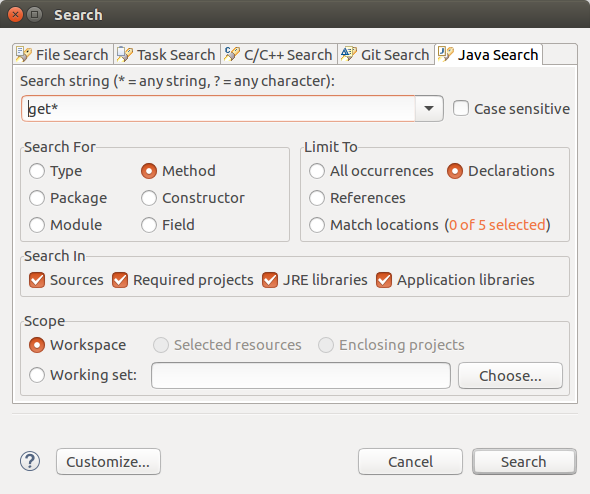
\includegraphics[width=8.5cm]{eclipse_suche.png}
\caption{Suchoption aus Eclipse}
\label{fig_sim}
\end{figure}



% Grafik in einer Spalte
\begin{figure}[!ht]
\centering
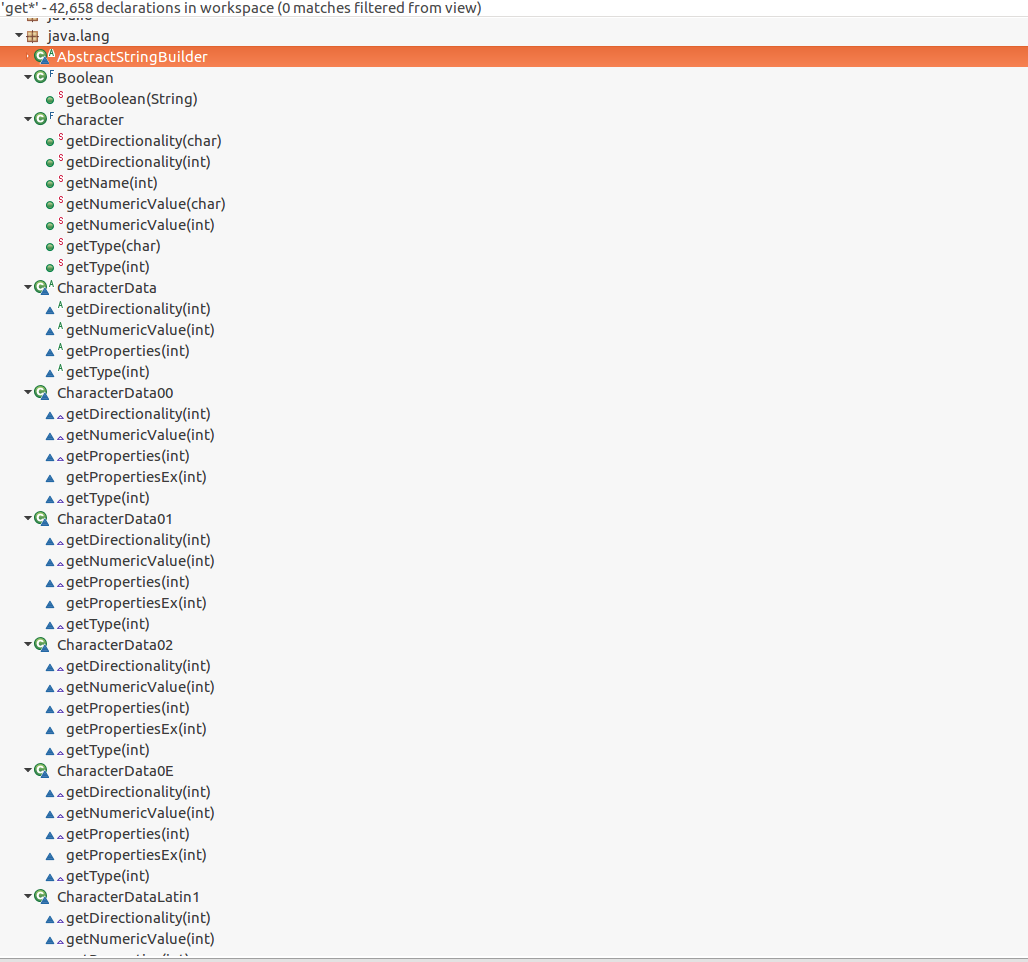
\includegraphics[width=8.5cm]{eclispe_suche_ergebniss.png}
\caption{Suchergebnis aus Eclipse}
\label{fig_sim}
\end{figure}


Daher ist für den Entwickler einfacher sich in einer API zurecht zu finden, wenn dessen Schnittstellen eine gewisse Konvention folgen \cite{haase2015}. 


\subsection{Keine redundanten Methoden}

Hier soll es aufzeigen, wieso man nicht für alles eine Methode schreiben sollte, wie z.B. beim einlesen von einem Images.


\subsection{Refactoring}\label{refactorL}

Das Refactoring beschreibt laut Fowler einen Prozess, bei dem bestehender Quellcode so verändern wird, dass es für denjenigen, der diesen Quellcode nutzt, keinen Einfluss haben wird  \cite{fowler1999}. Mit Das Refactoring wird versucht bestehenden Quellcode so zu verbessern, dass die Chancen minimiert werden, dass an einigen Stellen Programmfehler auftreten. Zudem wird meist Zusätzlich auch der Quellcode verbessert, so dass es besser lesbar und somit wartbar ist. Nach Fowler ist das Refactoring keine zusätzliche Arbeit, sondern ein fester Bestandteil bei der Software Entwicklung.

Auch wenn ein gutes Design der API vorliegen sollte, kann es bei zusätzlichen Erweiterungen dazu kommen, dass die Schnittstellen nicht mehr nach dem ursprünglichen Prinzip Designt worden sind. So könnte eine Namenskonvention nicht eingehalten worden sein \ref{MNP}. Es kann auch vorkommen, dass die Namen der Parameter einer Methode nicht aussagekräftig genug sind und dies zur Verwirrung führen könnte. Falls die API noch nicht veröffentlicht wurde, ist es zudem auch möglich die Schnittstellen selber neu zu beschreiben. 

Das Refactoring kann dazu genutzt werden, solche vorhandene Missstände auszubessern und den Quellcode leserlicher und für den Entwickler, der diese API nutzt, den Stress zu lindern. 
 
Als Beispiel soll folgende,sehr simple gehaltene, Schnittstelle dienen.
 
\begin{lstlisting}[language=Java,caption=Beispiel einer unleserliche Methode]

public void foo(int[] a, int[] b);

\end{lstlisting}

Der Name der Methode 

--TODO--
\section{Tools zur Unterstützung der Entwicklung einer API}

Bei dem Entwickeln einer API kann es sehr langwierig sein diese zu Programmieren und zu Testen. Viele Bibliotheken haben mehrere tausende Schnittstellen, was zu sehr unübersichtlichen Code führen kann. Es gibt allerdings viele Tools, die einem das Arbeiten erleichtern. Im Folgenden werden einige Tools vorgestellt und dessen Vorteile dargestellt. 


\subsection{Entwicklungsumgebung}\label{IDE}

Es gibt sehr viele Entwicklungsumgebungen, mit dessen Hilfe Programmiert werden kann. Einer der Bekanntesten Vertreter wäre Microsoft Visual Studio \footnote{https//www.visualstudio.com/}, welches es in vielen Verschiedenen Versionen gibt, Als Kostenpflichtige Premium Edition oder als kostenlose Community Edition. Sie bietet Unterstützung für viele verschiedene Programmiersprachen, wie C, C++, C\#, Javascript oder Python.
 
Neben der Entwicklungsumgebungen von Microsoft gibt auch noch IntelliJ von JetBrains\footnote{https://www.jetbrains.com/idea/}. Ähnlich wie Microsofts Visual Studio bietet IntelliJ Sprachunterstützung für viele verschiedene Programmiersprachen an. Auch gibt es hier ähnliche Modelle für den Entwickler, mit denen er Programmieren kann, von einer Kostenpflichtige als auch einer Kostenlosen. Im Gegensatz zu Microsoft Visual Studio ist IntelliJ auch außerhalb von Microsoft Windows Verfügbar. 

Die beliebteste Entwicklungsumgebung laut \ac{PYPL} ist das in Java geschriebene Programm Eclipse von Eclipse Software \footnote{http://www.eclipse.org/} \footnote{http://www.eclipse.org/}. Auch Eclipse erlaubt mithilfe von Erweiterungen eine Sprachunterstützung von unterschiedlichen Sprachen, ursprünglich war sie dabei allerdings nur für die Programmiersprache Java Gedacht. All die genannten Entwicklungsumgebungen unterstützen das Refactoring \ref{refactorL}. 

Entwicklungsumgebungen sind eine große Hilfe beim Entwickeln und verbessern einer API. Da die Entwickler meist über eine Entwicklungsumgebung auf eine API zugreifen, kann man leicht nachverfolgen, wie die natürliche Arbeitsweise eines Entwicklers ist der diese API nutzt. 

In vielen Entwicklungsumgebungen haben die Entwickler die Möglichkeit die Texteingabe Automatisch zu vervollständigen. So werden zum Beispiel bei der Eingabe von get in Eclipse mithilfe von den Tasten STRG und LEERTASTE unter anderem sämtliche Methoden aufgelistet, auf die der Entwickler Zugreifen kann. So hat der Entwickler jederzeit die Möglichkeit nach einer Methode zu suchen, die sein aktuelles Problem lösen kann. Dies hat den Vorteil, dass so überprüft werden kann, wie der natürliche verlauf von vielen Entwickler beim Entwickeln ist und wie die Entwickler mit einer API zurechtkommt. 


\subsection{Das Programm Checkstyle}

Nach fortschreitender Entwicklungszeit einer API kann es immer wieder mal zu nicht Konvention Gerechter Benennung der Schnittstellen kommen. Das kann nach Veröffentlichung der Schnittstelle dazu führen, dass die API es den Entwicklern erschwert, nach einer Schnittstelle zu suchen, die ihr Problem lösen könnte. Was wiederum dazu führen könnte, dass sie die Probleme selbst versuchen zu lösen, und es so zu undurchschaubaren Code kommen kann \footnote{http://checkstyle.sourceforge.net/}. 

Mithilfe von Checkstyle lässt sich der Quellcode automatisiert analysieren, um so die Konvention einzuhalten. Was genau alles überprüft wird und wie, wird in einer \ac{XML} Datei festgelegt. 

\begin{lstlisting}[language=Java,caption=Auszug einer XML Datei]

[...]
<module name="Checker">
    <module name="JavadocPackage"/>
    <module name="TreeWalker">
        <module name="AvoidStarImport"/>
        <module name="ConstantName"/>
        <module name="EmptyBlock"/>
    </module>
</module>
[...]

\end{lstlisting}


\section{Fazit}

Hier soll es nochmal einen Bezug auf die vorherigen Loesungsbeispielen geben und was für Vorteile es einem bringt.

%% --------------------------------------------------------------------

\section*{Abkürzungen}
\addcontentsline{toc}{section}{Abkürzungen}

\begin{acronym}
\acro{API}{\ Application Programming Interface}
\acro{HTML}{\ Hypertext Markup Language}
\acro{JDK}{\ Java Development Kit}
\acro{LWJGL}{\ Lightweight Java Game Library}
\acro{PYPL}{\ PopularitY of Programming Language}
\acro{SDK}{\ Software Development Kit}
\acro{STL}{\ Standard Template Library}
\acro{XML}{\ Extensible Markup Language}

\end{acronym}

% Literaturverzeichnis
\addcontentsline{toc}{section}{Literatur}
\printbibliography

\end{document}